%! Author = melek
%! Date = 9.06.2022

% Preamble
\documentclass[11pt]{article}

% Packages
\usepackage{amsmath}
\DeclareMathOperator*{\argmax}{argmax}

\usepackage{graphicx}
\usepackage{amssymb}
\graphicspath{ {../images/} }

% Document
\begin{document}

    \maketitle
    \setcounter{section}{5}


    \section{Exercises}

    \subsection{Question}
    If V changes during the episode, then (6.6) only holds approximately;
    what would the difference be between the two sides?
    Let V t denote the array of state values used at time t in the TD error (6.5) and in the TD update (6.2).
    Redo the derivation above to determine the additional amount that must be added to the sum of TD errors in order to equal the Monte Carlo error.

    \subsection*{Answer}

    If V is updated during the episode, which is the case for TD algorithm, it only makes difference if a state is visited more than once in an episode.

    Equation (6.2) becomes:

    $V_{t+1}(S_t) = V_t(S_t) + \alpha [ R_{t+1} + \gamma V_t(S_{t+1}) -V_t(S_t) ]$

    $V_{t+1}(S_t) = V_t(S_t) + \alpha \delta_t$

    Equation (6.5) becomes:

    $ \delta_t = R_{t+1} + \gamma V_t(S_{t+1}) - V_t(S_t) $

    Monte Carlo error is:

    $G_t-V(S_t) = R_{t+1} + \gamma G_{t+1} - V_t(S_t) = \delta_t + \gamma (G_{t+1} - V_t(S_{t+1})) $

    With updated values:

    $G_t-V(S_t) = \delta_t + \gamma (G_{t+1} - V_{t+1}(S_{t+1}) + \alpha \delta_{t-a}) $ where $a \nless 0$ indicates when the last update was.

    Note that if a state is visited only once then updated value is never used thus wen say that $V_t$ is similar to $V_{t+1}$.


    For simplicity lets assume a state can only be revisited just after visiting the state.
    We can introduce an indicator function denoted by f which returns 0 if a state is visited only once and 1 if it is visited again in next step.

   $G_t-V(S_t) = \delta_t + \gamma (G_{t+1} - V_{t+1}(S_{t+1}) + \alpha \delta_t f(S_t)) $

    Continue with the derivation:

    $G_t-V(S_t) = \delta_t + \gamma \alpha \delta_t f(S_t) + \gamma (G_{t+1} - V_{t+1}(S_{t+1})) $

    $G_t-V(S_t) = \delta_t + \gamma \alpha \delta_t f(S_t) + \gamma (  \delta_{t+1} + \gamma \alpha \delta_{t+1} f(S_{t+1}) + \gamma (G_{t+2} - V_{t+2}(S_{t+2})) ) $

    $G_t-V(S_t) = \sum_{k=t}^{T-1} \gamma^{k-t} \delta_k + \alpha \gamma \sum_{k=t}^{T-1} \gamma^{k-t}  \delta_t f(S_t)$

    \subsection{Question}

    This is an exercise to help develop your intuition about why TD methods are often more efficient than Monte Carlo methods.
    Consider the driving home example and how it is addressed by TD and Monte Carlo methods.
    Can you imagine a scenario in which a TD update would be better on average than a Monte Carlo update?
    Give an example scenario—a description of past experience and a current state—in which you would expect the TD update to be better.
    Here’s a hint: Suppose you have lots of experience driving home from work.
    Then you move to a new building and a new parking lot (but you still enter the highway at the same place).
    Now you are starting to learn predictions for the new building.
    Can you see why TD updates are likely to be much better, at least initially, in this case?
    Might the same sort of thing happen in the original scenario?

     \subsection*{Answer}

    TD updates bootstrap which means previous estimates are used.
    Considering the new home case, TD only needs to learn about states from the new home to the highway entrance.
    Remaining states are already known.
    MC updates cannot make use of current experience.
    MC will sample new complete episodes and at the beginning they will be very noisy.


     \subsection{Question}

    From the results shown in the left graph of the random walk example it appears that the first episode results in a change in only V (A).
    What does this tell you about what happened on the first episode?
    Why was only the estimate for this one state changed?
    By exactly how much was it changed?

    \subsection*{Answer}

    It appears first episode ended through state A\@.

    TD bootstraps which means it relies on previous estimates.
    All states are initialized to 0.5.
    This is an un-discounted task with $\alpha=0.5$.

    Let's remember equation (6.2):

    $V_{t+1}(S_t) = V_t(S_t) + \alpha [ R_{t+1} + \gamma V_t(S_{t+1}) -V_t(S_t) ]$
    \newline

    For all state changes except state A, V(S) is:

    $V_{t+1}(S_t) = V_t(S_t) + \alpha [ R_{t+1} + \gamma V_t(S_{t+1}) -V_t(S_t) ] = 0.5 + 0.1 [0 + 0.5 - 0.5] $

    $V_{t+1}(S_t) = 0.5 $ which indicates state values remain unchanged.
    \newline

    For change from state A to the terminal state, V(A) is:

    $V_{t+1}(S_t) = V_t(S_t) + \alpha [ R_{t+1} + \gamma V_t(S_{t+1}) -V_t(S_t) ] = 0.5 + 0.1 [0 + 0 - 0.5] $

    $V_{t+1}(S_t) = 0.45 $


    \subsection{Question}

    The specific results shown in the right graph of the random walk example are dependent on the value of the step-size parameter, $\alpha$.
    Do you think the conclusions about which algorithm is better would be affected if a wider range of $\alpha$ values were used?
    Is there a different, fixed value of $\alpha$at which either algorithm would have performed significantly better than shown?
    Why or why not?

    \subsection*{Answer}

    For all experienced $\alpha$ values TD performs better than MC.
    Using wider range of $\alpha$ would result in the same behaviour.

    Smaller $\alpha$ values may decrease the RMS error for both algorithm while making the learning very slow.
    Larger $\alpha$ values tends to speed up learning while increasing the RMS Error for both algorithms.

    \subsection{Question}

    In the right graph of the random walk example, the RMS error of the TD method seems to go down and then up again, particularly at high $\alpha$’s.
    What could have caused this?
    Do you think this always occurs, or might it be a function of how the approximate value function was initialized?

    \subsection*{Answer}

    All states are initialized with the same values.
    States with actually larger values takes positives updates.
    States with actually smaller values takes negative updates.
    This trend continues even after optimal values are reached and thus leads to error.
    This behaviour is especially visible for larger $\alpha$ values because they cause larger updates thus larger errors.

    Solution to this problem is to use random initialization of states.

    \subsection{Question}

    In Example 6.2 we stated that the true values for the random walk example are 1/6 , 2/6 , 3/6 , 4/6 , and 5/6 , for states A through E.
    Describe at least two different ways that these could have been computed.
    Which would you guess we actually used?
    Why?

    \subsection*{Answer}

    First solution would be to use dynamic programming with tabular updates.

    Second solution would be to use linear algebra to find state values.

    Equation 3.14:

     \begin{equation}
        v_{\pi}(s) = \sum_a \pi(a|s) \sum_{s',r} p(s',r| s,a) [r+\gamma v_{\pi}(s')]
    \end{equation}

    At each state neighbour states are selected with a probability of 1/2.
    Transitions occur with a probability of 1.
    This is a non-discounted problem.
    Equation 3.14 becomes:

    \begin{equation}
        v_{\pi}(s) = \sum_a 0.5 [r+ v_{\pi}(s')]
    \end{equation}

    For each state this equation can be used:
    \newline

    $ v(A) = 0.5 [0+ v(Term)] + 0.5 [0+ v(B)] = 0.5*v(B) $

    $ v(A) - 0.5*v(B) = 0 $
    \newline

    $ v(B) = 0.5 [0+ v(A)] + 0.5 [0+ v(C)] = 0.5*v(A) + 0.5*v(B) $

    $ v(B) - 0.5*v(A) - 0.5*v(B) = 0 $
    \newline

    $ v(C) = 0.5 [0+ v(B)] + 0.5 [0+ v(D)] = 0.5*v(B) + 0.5*v(D) $

    $ v(C) - 0.5*v(B) - 0.5*v(D) = 0 $
    \newline

    $ v(D) = 0.5 [0+ v(C)] + 0.5 [0+ v(E)] = 0.5*v(C) + 0.5*v(E) $

    $ v(D) - 0.5*v(C) - 0.5*v(E) = 0 $
    \newline

    $ v(E) = 0.5 [0+ v(D)] + 0.5 [1+ v(Term)] = 0.5*v(D) $

    $ v(E) - 0.5*v(D) = 0.5 $
    \newline


    This equations can be written in matrix form:

    \begin{bmatrix}
1 & -0.5 & 0 & 0 & 0\\
-0.5 & 1 & -0.5 & 0 & 0\\
0 & -0.5 & 1 & -0.5 & 0\\
0 & 0 & -0.5 & 1 & -0.5\\
0 & 0 & 0 & -0.5 & 1
\end{bmatrix} *  \begin{bmatrix}
V(A)\\
V(B)\\
V(C)\\
V(D)\\
V(E)
\end{bmatrix} =
    \begin{bmatrix}
0\\
0\\
0\\
0\\
0.5
\end{bmatrix}
\newline

    This system of linear equations can be solved using linear algebra.

    \subsection{Question}

    Design an off-policy version of the TD(0) update that can be used with arbitrary target policy $\pi$ and covering behavior policy b, using at each step t the importance sampling ratio $\rho_{t:t}$  (5.3).

    \subsection*{Answer}

    Equation 5.4 shows how state value function is defined in the off-policy case.

    $ E[  \rho_{t:T-1} G_{t} | S_t=s ] = v_{\pi}(s) $
    \newline

    TD(0) update rule from 6.2 is:

    $V(S_t) = V(S_t) + \alpha [ R_{t+1} + \gamma V(S_{t+1}) -V(S_t) ]  $
    \newline

    In the off-policy case, the update rule becomes:

    $V(S_t) = V(S_t) + \alpha [ \rho_{t:t} ( R_{t+1} + \gamma V(S_{t+1}) ) -V(S_t) ]  $

    \subsection{Question}

    Show that an action-value version of (6.6) holds for the action-value form of the TD error t = R t+1 + Q(S t+1 , A t+1 ) Q(S t , A t ), again assuming that the values don’t change from step to step.

    \subsection*{Answer}

    $ G_t-Q(S_t,a_t) = R_{t+1} + \gamma G_{t+1} - Q(S_t,a_t) + \gamma Q(S_{t+1},a_{t+1}) - \gamma Q(S_{t+1},a_{t+1}) $
    \newline
    $ G_t-Q(S_t,a_t) = \delta_t + \gamma (G_{t+1} - Q(S_{t+1},a_{t+1}) ) $
    \newline
    $ G_t-Q(S_t,a_t) = \delta_t + \gamma \delta_{t+1} + \gamma^2 (G_{t+2} - Q(S_{t+2},a_{t+2}) )  $
    \newline
    $ G_t-Q(S_t,a_t) = \vdots$
    \newline
    $ G_t-Q(S_t,a_t) =  \sum_{k=t}^{T-1} \gamma^{k-t} \delta_k  $

    \subsection{Question}

    Windy Gridworld with King’s Moves (programming) Re-solve the windy gridworld assuming eight possible actions, including the diagonal moves, rather than the usual four.
    How much better can you do with the extra actions?
    Can you do even better by including a ninth action that causes no movement at all other than that caused by the wind?

    \subsection*{Answer}

    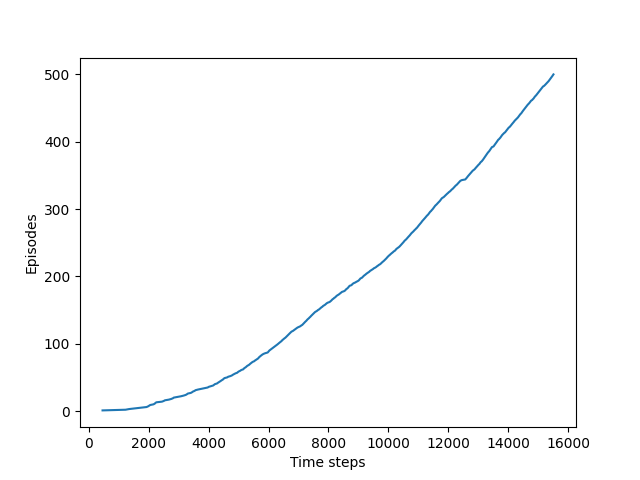
\includegraphics[scale=0.4]{figure_6_3}
    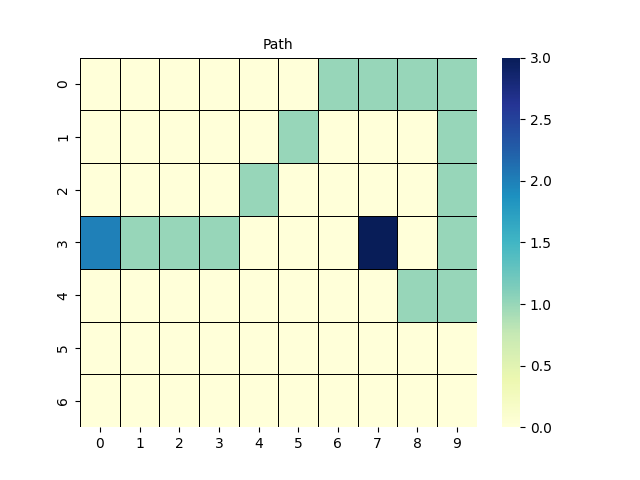
\includegraphics[scale=0.4]{figure_6_3_grid}

    Regular 4 actions.

    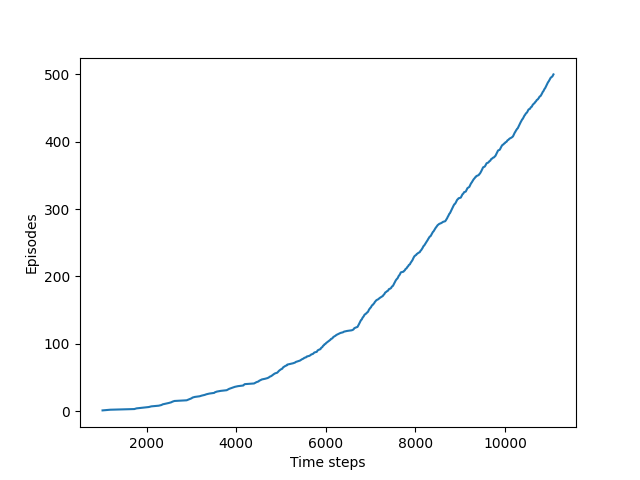
\includegraphics[scale=0.4]{figure_6_3_ex_6_9_a}
    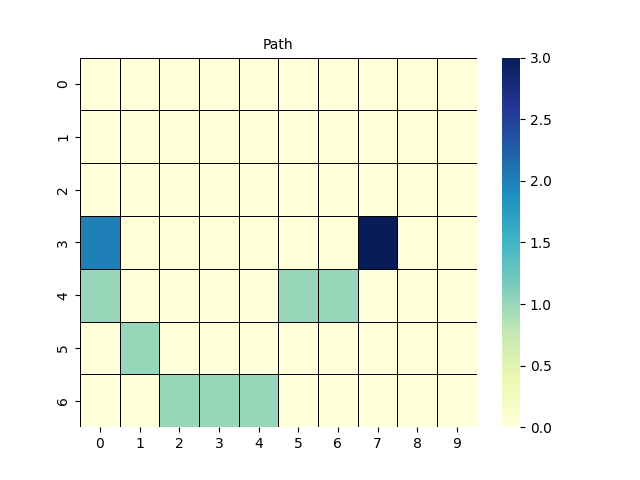
\includegraphics[scale=0.4]{figure_6_3_ex_6_9_a_grid}

    8 actions.
    Episode lengths became significantly shorter than the regular 4 actions.

    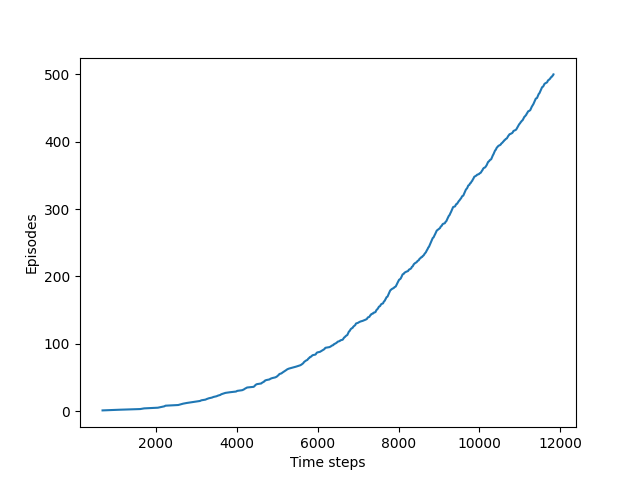
\includegraphics[scale=0.4]{figure_6_3_ex_6_9_b}
    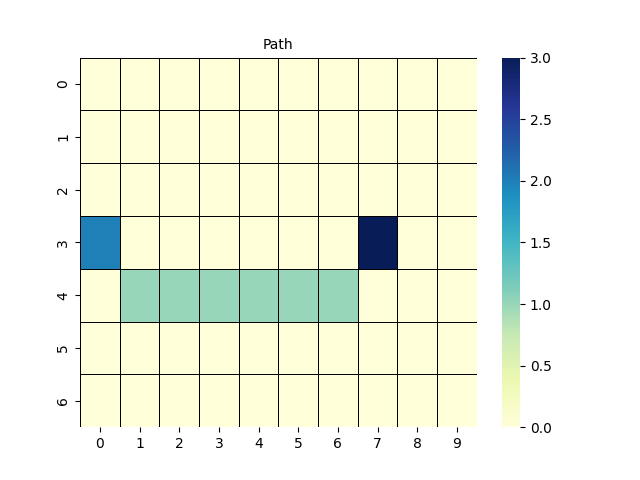
\includegraphics[scale=0.4]{figure_6_3_ex_6_9_b_grid}

    9 actions.
    Episode lengths became shorter than the regular 4 actions case but longer than the 8 actions case.

    \subsection{Question}

    Stochastic Wind (programming) Re-solve the windy gridworld task with King’s moves, assuming that the e↵ect of the wind, if there is any, is stochastic, sometimes varying by 1 from the mean values given for each column.

    \subsection*{Answer}

    Adding stochastic steps increased episode lengths dramatically.

    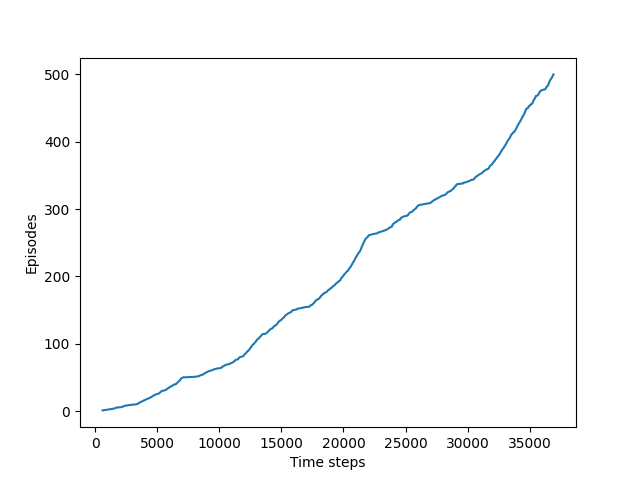
\includegraphics[scale=0.4]{figure_6_3_ex_6_10}
    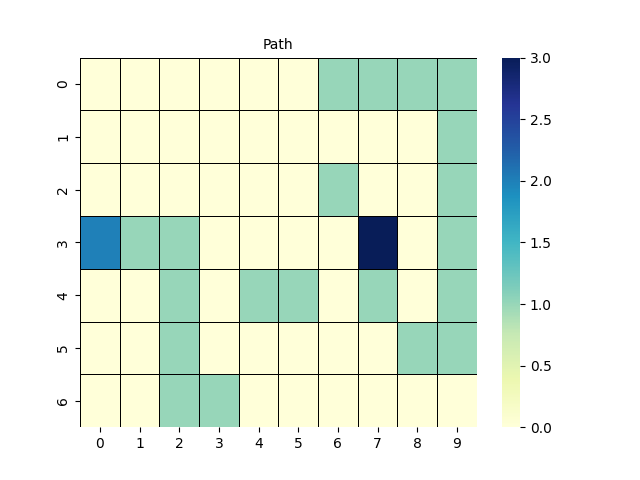
\includegraphics[scale=0.4]{figure_6_3_ex_6_10_grid}

    \subsection{Question}

    Why is Q-learning considered an off-policy control method?

    \subsection*{Answer}

    off-policy methods evaluate or improve a policy different from that used to generate the data.

    In Q-learning actions generated using a policy derived from Q e.g. using $\epsilon-greedy$.
    Updates are generated using max function with respect to current Q function.

    \subsection{Question}

    Suppose action selection is greedy.
    Is Q-learning then exactly the same algorithm as Sarsa?
    Will they make exactly the same action selections and weight updates?

    \subsection*{Answer}

    The update rules become similar.
    However, the algorithms are different.
    In SARSA the action used in update rule is used again in next loop.
    In Q-learning the action in update rule is not used again in next loop.
    Newly selection action, even-tough it is selected greedily, it may be different because Q function is updated.

    \subsection{Question}

    What are the update equations for Double Expected Sarsa with an $\epsilon$-greedy target policy?

    \subsection*{Answer}

    Equation 6.9 gives update rule for expected SARSA.
    \newline

    $ Q(S_t, A_t) =  Q(S_t, A_t) + \alpha [ R_{t+1} + \gamma E_{\pi} [ Q(S_{t+1}, A_{t+1}) | S_{t+1}] - Q(S_t, A_t) ] $
    \newline

    In double expected SARSA there will be two policy to select actions $\pi_1$ and $\pi_2$  with their respective action value functions $Q_1$ and $Q_2$.
    \newline

    $ Q_1(S_t, A_t) =  Q_1(S_t, A_t) + \alpha [ R_{t+1} + \gamma E_{\pi_2} [ Q_2(S_{t+1}, A_{t+1}) | S_{t+1}] - Q_1(S_t, A_t) ] $
    \newline

    $ Q_2(S_t, A_t) =  Q_2(S_t, A_t) + \alpha [ R_{t+1} + \gamma E_{\pi_1} [ Q_1(S_{t+1}, A_{t+1}) | S_{t+1}] - Q_2(S_t, A_t) ] $


    \subsection{Question}

    Describe how the task of Jack’s Car Rental (Example 4.2) could be reformulated in terms of afterstates.
    Why, in terms of this specific task, would such a  reformulation be likely to speed convergence?

    \subsection*{Answer}

    In car rental problem next state is known after moving some number of cars from one car park to another.
    Having 4 cars and moving 2 cars would result in 6 cars in a car park.
    Also having 5 cars and moving 1 car would result in 6 cars in a car park.
    Both state action pairs should have the same value.
    Instead the problem can be formulated using after states such that the car park starts the day with 6 cars without considering how many cars moved.

    Such reformulation is likely to speed convergence because number of states to evaluate is decreased.
    Number of cars moved is removed from the equation thus much fewer samples are needed.




\end{document}


